\input{wsc15style.tex}     % download from author kit.  Style files for wsc formatting. Don't remove this line - required for generating the final paper!

\documentclass{wscpaperproc}
\usepackage{latexsym}
\usepackage{caption}
\usepackage{graphicx}
\usepackage{mathptmx}
\usepackage[utf8]{inputenc}


%****************************************************************************
%% AUTHOR: You may want to use some of these packages. (Optional)
%\usepackage{amsmath}
%\usepackage{amsfonts}
%\usepackage{amssymb}
%\usepackage{amsbsy}
%\usepackage{amsthm}

\usepackage{algorithm,algorithmicx,algpseudocode}
\usepackage{float}
\usepackage{booktabs}
 \usepackage{multirow}



\algnewcommand\And{\textbf{and}}

\usepackage{mathtools}
\DeclarePairedDelimiter\abs{\lvert}{\rvert}%
\DeclarePairedDelimiter\norm{\lVert}{\rVert}%

\newcommand{\specialcell}[2][c]{%
  \begin{tabular}[#1]{@{}c@{}}#2\end{tabular}}


\makeatletter
\let\oldabs\abs
\def\abs{\@ifstar{\oldabs}{\oldabs*}}
\let\oldnorm\norm
\def\norm{\@ifstar{\oldnorm}{\oldnorm*}}
\makeatother

\usepackage{xcolor}
    \usepackage{cite}


\newcommand{\memo}[2]{\textcolor{#1}{#2}}
\newcommand{\added}[2]{\textcolor{#1}{#2}}
%\renewcommand{\memo}[2]{} % uncomment in the final version
%\renewcommand{\added}[2]{#2} % uncomment in the final version
\newcommand{\todo}[1]{\memo{red}{TODO: #1\\}}
\newcommand{\simon}[1]{\memo{green}{Simon: #1\\}}
\newcommand{\jm}[1]{\memo{blue}{JM: #1\\}}
\newcommand{\xrc}[1]{\memo{orange}{XRC: #1\\}}
\newcommand{\new}[1]{\added{orange}{#1}}

\begin{document}

\WSCpagesetup{Montanier, Carrignon, Rubio and Zerr}

\title{Modelling the co-evolution of trade and culture in the Roman market}

\maketitle

\begin{figure*}[htb]
{
\centering
Jean-Marc Montanier\\
Simon Carrignon\\ 
Xavier Rubio-Campillo\\
\vspace{12pt}
Barcelona Supercomputing Center\\
Carrer de Jordi Girona, 29, \\
08034 Barcelona, Spain\\
}
\end{figure*}


\section*{ABSTRACT}

\todo{Rewrite later}
In this article our aim is to present a model suitable to test various hypotheses on economic and cultural co-evolution during the Roman Empire. The ultimate goal is to address debates from history of economy such as the type of economical market found in early empires. Agent based modelling is a good way to understand social self-organisation resulting from a large number of interactions. It is used in a wide range of fields of research, from economical market mechanisms to social dynamics. We therefore apply this type of framework to our study.

Here we present a model able it reproduces well known economical and cultural mechanism. Moreover this model can be envisioned to test hypothesis on those mechanisms. Given the appropriate match between the simulations and archaeological and historical data, the results of the model can be validated.


\section{INTRODUCTION}\label{sec:intro}

% the spread of cultural traits is often modelled following neutral theory

Cultural change comprise the collection of processes that promotes or inhibits the spread of information by social interaction within a population~\shortcite[3]{boyd_origin_2005}. An increasing number of social scientists are using an evolutionary framework to model these dynamics, thus fostering the development of transdisciplinary efforts designed to understand cultural evolution~\shortcite{henrich_evolution_2003}.

Several studies focus on the biases that affect the transmission of cultural traits, including the relevance of intrinsic traits and frequency dependence properties. These analysis often compare evidence against neutral models~\shortcite{neiman_stylistic_1995}. They assume that traits do not affect the fitness of the individual that acquire it; within this context its transmission is unbiased, and its success will depend on its popularity amongst the rest of individuals. This neutral model generates a distinctive pattern of frequency distribution of traits, identified as a power law. It can be replicated with a simple random copying transmission mechanism~\shortcite{bentley_random_2004}: an individual will copy the traits of a randomly chosen individual with a given probability. This copy can potentially introduce some errors in the acquired trait, which account for innovation processes. The individual will in turn continue to spread these cultural traits which will be further adopted by other individuals. This basic model can be enriched by several additional processes both in the innovation~\shortcite{schillinger_copying_2014,sole_evolutionary_2013,ziman_technological_2003} and the transmissio~\shortcite{heyes_social_1994,henrich_evolution_2003}. Unbiased transmission works as a baseline for identifying frequency-dependent biases: if evidence has higher tendendy to copy the most common trait is is known as conformism, while the opposite is defined as anti-conformism.

This approach can be used as the starting point to analyse patterns of cultural change to explore frequency-dependance in archaeological contexts~\shortcite{lipo_neutralitystyle_2001,shennan_ceramic_2001,steele_ceramic_2010}. However, the fact that archaeology records fragmented material culture presents some challenges on the validity of the method~\shortcite{kandler_nonequilibrium_2013,porcic_exploring_2014,crema_approximate_2014}.

This work explores the impact of a crucial element on the transmission of material culture: trade. Networks of good exchanges are being increasingly recognised as key elements that structured ancient societies~\shortcite{temin_market_2001,remesal_epnet_2014,brughmans_connecting_2010}. The scenarios where this process emerge suggest a complex bias in the selection of cultural traits, which at the same time are also identified as economic products~\shortcite{bentley_specialisation_2005,macmillan_agent-based_2008}. Trasmission is not neutral anymore, as different prices for each product will introduce a dynamic content bias. This affects the frequency of the product within the population, which in turn would modifies its price following a co-evolutionary dynamic.

This work explores these co-evolutionary dynamics using a theoretical Agent-Based Model (ABM), a type of simulation particularly useful for studying non-linear dynamics in heterogeneous environments within an evolutionary perspective~\cite{lake_trends_2014}. Next section defines the model, which is based on unbiased transmission mechanisms and simple exchange dynamics. Next, we define different experiments to explore the dynamics of the created model. Finally, the concluding remarks interpret the results and discuss further possibilities of the pesented model.

\section{MODEL DESCRIPTION}

The model is composed of a population $Pop$ of $m$ agents, each defined by 2 vectors of size $n$. The first corresponds to the quantity of each good that the agent $i$ possesses: 
$$\forall i \in Pop, \quad Q^i = (q^i_1,\cdots,q^i_n) $$

where $Q^i$ is the total list of possessions of agent $i$, and $q^i_j$ is the number of goods of type $j$ that agent $i$ posses.

The second vector reflects the estimation of the value of a product that an agent $i$ makes.
$$\forall i \in Pop, \quad V^i = (v^i_1,\cdots,v^i_n) $$
where $V^i$ is the total list of estimated values of agent $i$, and $v^i_j$ is the value that agent $i$ associates to the goods of type $j$.

On top of these elements four processes are used: \emph{production}, \emph{cultural transmission}, \emph{innovation} and \emph{trade}. The \textit{production} process describes the creation of goods by the agent. Once a good is produced by an agent $i$ it is added its quantity vector ($Q^i$). The \emph{trade} process models the exchange of goods between the agents which results in a modification of the quantity vectors ($Q^i$). The amount of goods exchanged is computed by the agents concerned by the trade, within the \emph{trade} process, based on their value vectors ($V^i$). Within the \textit{cultural transmission} process an agent $i$ can copy the value vector ($V^j$) of an agent $j$, where $j \neq i$. The \textit{innovation} process also modifies the value vector $V^i$ of an agent, but it differs from the \emph{cultural transmission} process in that the modification is done without reference to the other agents. Finally, .

The scheduling of the four processes is described in algorithm~\ref{algo:complete} along with the vectors modified by each of these processes. Between line 2 and 7 all agents of the population are initialised with empty quantity vectors and random values. Between the lines 11 and 19 is presented the part of the pseudo-code describing the instructions that will be repeated for each iteration of the simulation. 
\jm{what about saying that we just count the iterations at the ``imitation, innovation step" ?}
\xrc{It should be justified (market is faster than cultural change?)}
One can note that the trading process is performed at every iteration while the imitation and innovation processes are executed only every $CulturalStep$. The idea behind this is to perform the imitation based on a score that reflects the performance of the agent and not only one lucky or unlucky trading round. 

\begin{algorithm}
\caption{Model}
\label{algo:complete}
	\begin{algorithmic}[1]
	\scriptsize
	\State INITIALIZATION: 
		\For{$j \in Goods$}
			\For{$i \in \#Pop/\#Goods$} \Comment{Initialize the agent with no products and a random value vector}
				\State $Q^i = (0, \cdots, 0)$
				\State $V^i = (v^i_0, \cdots, v^i_n)$ \Comment{The values of $v^i_j$ are selected randomly}
			\EndFor
		\EndFor

	\State SIMULATION:
		\Loop{$~step \in TimeSteps$}
			\For{$i \in Pop$}
				\State $Production(Q^i)$
				\For{$j \in Pop$}
					\State $TradeProcess(V^i,Q^i,V^j,Q^j)$
				\EndFor				
				\If{$ (step \mod CulturalStep) = 0$}	
					\State $CulturalTransmission(V)$
					\State $Innovation(V^i)$
				\EndIf
			\EndFor
		\EndLoop
\end{algorithmic}
\end{algorithm}


In order to validate our model we first reproduce common results from the literature on cultural transmission. We then show that it is possible to transform our model to fit processes that are economically sound. To achieve these two goals, we have design for each one specific set of implementations of the four core processes (production, imitation and innovation). 

\subsection{Cultural Transmission}\label{sec:culturalTrans}

The first set of implementations is designed to reproduce a scenario of unbiased transmission, where each product is a cultural trait without intrinsic positive or negative weight \shortcite{bentley_random_2004,bentley_specialisation_2005,mesoudi_random_2009}. 
Under this hypothesis, the processes of \emph{production} and \emph{trade} are not relevant, and as a consequence, they do not modify the content of the quantity vectors of the agents.

Unbiased transmission is implemented using ``random copy'': each agent has a low probability to pick randomly one agent among all and copy its vector of values. The \emph{innovation} process, termed ``unbounded'', is triggered with a low probability and draw a new random value to replace an element $v^i_j$. The imitation and innovation probabilities are presented with other parameters in table~\ref{tab:parameters}.

The neutral hypothesis states that the ``random copy'' transmission and the ``unbounded'' innovation process used under a fixed population size leads to a \emph{power law} distribution of the frequency for the different cultural variants. This distribution is characterized by a small number of very frequent traits and a large number of very rare traits. 
%Since this hypothesis has been verified in previous works implementing similar \emph{imitation} and \emph{innovation} mechanisms, we expect in this work the observation of a similar ``power law' distribution. 
More formally, this distribution is formalised as : $$P(v)=C/v^\alpha $$, where $v$ is the number of time a variant has been repeated, $P(v)$ the probability to find that variant, $C$ a constant, $\alpha$ a variable describing the slope of the curve obtained. 

\subsection{Trading Model}\label{sec:trade}

The second set of implementations of the core processes aims at producing economical dynamics. We are interested in the exchange of products between agents when they can modify the prices at which they sell and buy products. We want to implement simple processes leading to the convergence of all prices to values acceptable by all agents, i.e. we would like to observe, at the end of an experiment, all the agents using the same set of prices which allow them to trade efficiently.

\paragraph{Production}
In this set of implementations, each agent is producing only one type of good. The type good produced by an agent $i$ is assigned to it at the beginning of the simulation, does not change through the simulation and is referred as $produced^i$. 

\paragraph{Cultural transmission}
Within this set of implementations, the cultural transmission process is not random but biased toward the agents which are the best at trading, and is therefore termed ``success bias''. To achieve this bias, the cultural transmission mechanism used takes into account the value vector of the other agents and relies on two new notions: \emph{need} and \emph{score}. 

The \emph{need} is a quantity of product that each agent tries to obtain. This quantity is different for each product but the need for a product is the same for all agents:
$$ N = (n_1, \cdots, n_r) $$ 

The \emph{score} $s^i$ of an agent $i$ reflects the ability of this agent to obtain the products it needs. It is maximum when the quantity vector of an agent is equal to its need vector and lower proportionally to the distance between the need vector and the quantity vector.  It is formally computed as follow for agent $i$:

\begin{equation}\label{eq:score}
s^i = \begin{cases}
 s_{max}=1 & \text{if $q^i_j = n_j$}\\
1 -\dfrac{\abs{q^i_j - n_j}}{ \sqrt{\abs{(q^i_j)^2-(n_j)^2}}} & \text{if $q^i_j \neq n_j$}
\end{cases}
\end{equation}


This function ensures that each good has the same weight in the final score (i.e.: managing to get only the right amount of a good with a high ``need'' value will not give a better score to the agent).


\begin{figure}[htp]
	\begin{center}
		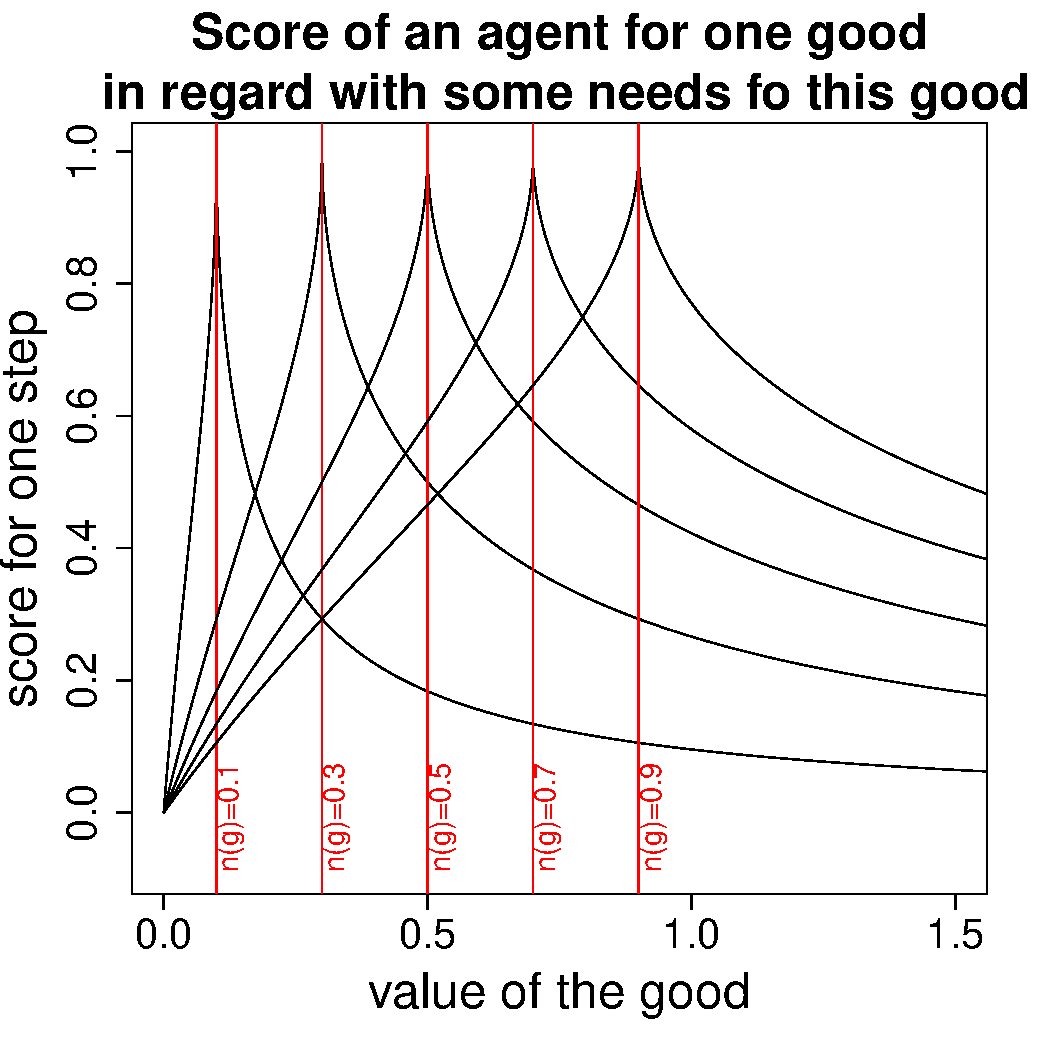
\includegraphics[width=7cm]{img/fitness.pdf}
	\end{center}
	\caption{The payoff depending on the estimated value and the effective needs $n(g)$ of a good.}
	\label{fig:fit}
\end{figure}
The figure~\ref{fig:fit} depicts the score of an agent, for different need value of one good, with regards to the quantity of the good possessed by the agent. We can see that even if the need for a good is small (for instance when $n(g) = 0.01$) an agent can have a high score as soon as it manages to get a quantity close to the need. This insures that an agent needs to have for each of the good a quantity equal to the need and that no agent could reach a better score just by getting the right quantity for a good with a high need.

The agents will choose the agent from whom the price vector should be copied among the agents that produce the same good and have the highest score. In practice, a fixed proportion of the less successful agents will copy the prices of the most successful agent. 


\paragraph{Trading} 
During the trading phase the value associated to a good by an agent corresponds to the subjective price of the good for this agent. Briefly summarised, for each good that it does not produce, an agent will trade with the first parter that offer an acceptable trade, i.e. the agent that proposes a satisfiable ratio between the other product and the product produced by the agent. 

In more details, the trading phase starts by the agent looking at a first random agent producing another product. 
Let $o$ be an agent producing $g$ that proposes a trade and $r$ an agent producing $k$ that receives the proposition. As explained earlier, each has a quantity of good $Q^o$ and $Q^r$. On the one side, $o$ wants to exchange a quantity $w_g^o$ of the good $g$ for a quantity $w_k^o$ of the good $k$. On the other side, $r$ wants to exchange a quantity $w_g^r$ of the good $g$ for a quantity $w_k^r$. The tuples $W^o$ and $W^r$ describe the quantities of goods wanted by agent $o$ and $r$ for one trade proposition and are defined by:  

\begin{equation}
	 W^o=(w_g^o = v_g^o,w_k^o= \frac{v_k^o}{v_g^o}) 
	 W^r=(w_k^r = v_k^r,w_g^r= \frac{v_g^r}{v_k^r}) 
	 \label{eq:trade}
\end{equation}

 Where $v_j^i$ are the estimated value of the good $j$ by the agent $i$ as defined earlier. 
The requested quantity of the non produced good is simply the ratio between the estimated value of the good requested and the estimated value of the produced good.


Once the quantities are defined, the agents declare that the trade is possible if :
\begin{align}
q_g^o >= w_g^o,\quad q_g^r <= w_g^o,\quad q_k^r >= w_k^o \label{eq:constraintQty}\\
w_g^o>=(q_g^r+w_g^r),\quad w_k^o<=w_k^r,\quad w_g^o<=w_g^r \label{eq:constraintWill}
\end{align}


The conditions \ref{eq:constraintQty} insure that both agents have enough goods in their inventory to realise the trade while the conditions \ref{eq:constraintWill} insure that the quantities of each good fit the will of both agents.



If a trade is possible the two agents will exchange the agreed quantities. If the trade is not possible, the agent will continue to look at random partners for this good until either a good is found or $TradeThreshold$ agents have been tried. At this point the agent will try to trade with agents producing another good. The process goes on until all goods have been tried. This trading process is described in algorithm~\ref{algo:trade}.

\begin{algorithm}
\caption{Trading Process for agent $o$}
\label{algo:trade}
	\begin{algorithmic}[1]
	\scriptsize
		\For{$j \in Goods \And j \neq produced^i $}
			\State $tradeAttempt = 0$
			\For{$r \in Pop \And produced^r = j \And tradeAttempt < TradeThreshold $}
				\If{$acceptableTrade(W_o,W_r)$}
					\State $trade(W_o,W_r)$
				\Else
					\State $tradeAttempt = tradeAttempt + 1$					
				\EndIf
			\EndFor
		\EndFor
\end{algorithmic}
\end{algorithm}


\paragraph{Innovation} In a trading environment it seems unlikely that a price will change radically to a very different value. Therefore, a new and more realistic mechanism is proposed. The innovation process, termed ``self referenced'', is still triggered with a probability $\mu$ 
but modify the previous price by adding or subtracting a small amount taken randomly from a uniform  distribution between $0 .. \beta$.


\paragraph{Expected outcome} 

Based on the set of implementations presented and given the equations (\ref{eq:score}) and (\ref{eq:trade}), it is expected that the prices will converge to value allowing each agent to obtain quantities of resources exactly equivalent to the needs. The best possible price of all good satisfies the equations :
\begin{equation}
	\begin{cases}
		\frac{v^o_k}{v^o_g} = n_k \\
		v^o_g = n_g 
	\end{cases} =>v^o_k = n_k \times n_g, \quad \forall k \in Goods, \forall o \in Pop, g = produced^o, k \not= g 
\end{equation}

Which means that 

\begin{equation}
	\quad \forall j \in Goods, \forall i \in Pop \quad \tilde{V}^i = 
	\begin{cases}
		\tilde{v}^i_j = n_j & \text{if $ j=produced^i$}\\
		 \tilde{v}^i_j = n_j \times n_{produced^i} & \text{else}
	\end{cases}\label{eq:optimum}
\end{equation}


If such prices are reached, given the exchange rules defined in (\ref{eq:trade}) and the exchange constraints (\ref{eq:constraintQty}) and (\ref{eq:constraintWill}) all exchanges will be optimally achieved, leading to a total score $S$ for each agent of the population : 
$$ S = \sum_{i=0}^{CulturalStep}  s^i(\tilde{Q}^i) \times ngoods $$ 
where $\tilde{Q}^i$ is the optimal quantity vector, i.e. the one for which $s^i(\tilde{Q}^i) = s_{max}$. Remember that from equation~\ref{eq:score}, $s_{max}=1$.

\section{Experimental setup}
%In order to study the cultural transmission and the trading model two sets of implementation of the four processes of our model have been presented. Remember that during the definition of these two sets of implementation, two cultural transmission mechanisms have been defined () along with two innovation mechanisms (). Therefore, on top of exploring the results offered by the two set of implementations, it would be also interesting to understand which of the process is responsible for the variation in results. The four implementations proposed are summarized in the table~\ref{tab:exp}. Each couple of innovation/imitation mechanism form one setup that is labelled with one letter. Note that the ``neutral model" presented in section~\ref{sec:culturalTrans} corresponds to the setup A, and the trading model presented in section~\ref{sec:trade} corresponds to the setup D.
%
%\begin{table}[h]
%	\centering
%	\begin{tabular}{ll|cc}
%				&	&\multicolumn{2}{c}{\textbf{Cultural transmission}} \\
%		\multirow{2}[20]{*}{\rotatebox[origin=c]{90}{\textbf{Innovation}}}&  & Random & Success biased \\\hline  
%		& \rule[-0.45cm]{0pt}{1cm} Unbounded 		&A & B \\
%		& \rule[-0.45cm]{0pt}{1cm} Self Referenced	& C & D \\
%	\end{tabular}
%	\caption{Experimental Setup}
%	\label{tab:exp}
%\end{table}

For the cultural transmission setup we run two set of experiments with 250 and 500 agents in which we vary $\alpha \in \{0.004,0.016,0.064\}$. For each combination of parameters we did 100 runs of 10000 timestep is performed. 

For the trading model we run  again two set of experiment, one with 2 goods and 500 agents, the other with 4 goods and 800 agents. The length of the simulations is always 10000 timestep but this time one timestep is made of $CulturalStep$ trade action as described in the previous section~\ref{sec:trade}. Again for each combination 100 runs are done.

The whole set of parameters used are presented in table~\ref{tab:parameters}. 

%Finally, remember that in our experiment one has to take in account that agents modifies their prices or exchange their price only every $culturalStep$ steps. Between, twos such steps, the agent exchange goods given their own prices. Therefore we choose to run our simulation during 10000 step which correspond the 1000 time steps used by \shortcite{bentley_random_2004,mesoudi_random_2009}.

\begin{table}
\begin{center}
\begin{tabular}{@{}ll@{}}
\toprule
Parameter & Value \\
\midrule
Number of goods & 4 \\
Number of agents & 800 \\
Mutation probability & .004 \\
Innovation probability & .001\\
CulturalStep &  10 \\
TradeThreshold & 100  \\
TimeSteps & 200000 \\
\bottomrule
\end{tabular}
\caption{Table of parameters}\label{tab:parameters}
\end{center}
\end{table}






\section{RESULTS}
\subsection{Random cultural transmission and random innovation process}

We first analyse the result obtained in the ``neutral model" as presented in section~\ref{sec:culturalTrans}.  The figure~\ref{fig:allMutation} present the results obtained with $\mu$ varying $\in {.004,.008,.016,.064}$ and two population sizes: 250 and 500 agents. The distribution of variants obtained is shown in figure~\ref{fig:allMutation}. In this graph the relative frequencies of the values obtained is analysed. The y-axis of the graph shows the frequencies of the variants of the vector values, the x-axis shows how many variant achieves such frequencies and the line represents the average of the frequencies obtained across all runs. Both axes are in a logarithmic scale.

\begin{figure}[!hbp]
	\begin{center}
		\includegraphics[width=6cm]{img/allmuRandMaxN250.pdf}
		\includegraphics[width=6cm]{img/allmuRandMaxN500.pdf}
	\end{center}
	\caption{Distribution of frequencies depending on the $\mu$ parameter with 250 agents (left) and 500 agents (right)\label{fig:allMutation}}
\end{figure}

In the figure~\ref{fig:allMutation} one can observe that the lower the mutation rate, the closer from a line the result is. This line corresponds to the ``power law" distribution explained in section~\ref{sec:culturalTrans} and is typical of the result obtained under the ``neutral model". Please note, that here the specific variant achieving high frequency is not studied, only the number of variants achieving such frequencies is presented.  

Under all parameters tested the value vectors exhibit power law like distribution. It would then be interesting to analyse the shape of such distribution. In order to perform this study a linear regression is used to fit the curve obtained to a function of the form $P(v)=C/v^\alpha $. The mean value of the $\alpha$ parameters obtained and their standard deviation is presented in table~\ref{tab:mualpha}.

\begin{table}[h]
	\centering
	\begin{tabular}{ll|llll}
		\multicolumn{2}{r}{Agents Number}&\multicolumn{2}{c}{Our result}&\multicolumn{2}{c}{Bentley et al 2004}\\
			&$\mu$ & $\alpha$ & SD&$\alpha$&SD\\\hline
		N = 250	&0.004&1.53&0.03&1.54&0.02\\
			&0.016&1.57&0.02&1.57&0.01\\
			&0.064&1.66&0.01&1.67&0.01\\\hline
		N= 500	&0.004&1.50&0.02&1.53&0.03\\
			&0.016&1.55&0.03&1.61&0.04\\
			&0.064&1.78&0.08&1.81&0.10\\
	\end{tabular}
	\caption{Mean \& SD are calculate on 100 run.}
	\label{tab:mualpha}
\end{table}

\jm{Simon, do you have a comment on the table ? Like does it fit what is found in other articles ?}

\subsection{Distribution}

In order to understand the effect of introduction of trading mechanisms we compare first the distribution of values obtained in the two models. The result of this comparison is in the figure~\ref{fig:2setDi}. 

\begin{figure}[H]
	\begin{center}
		\includegraphics[width=6cm]{img/2SetupDistrib.pdf}
	\end{center}
	\caption{Frequency distribution for the neutral and the trade models}
	\label{fig:2setDi}
\end{figure}


%\begin{table}[h]
%	\centering
%	\begin{tabular}{lcccc}
%		& A & B & C & D\\
%A & X& \includegraphics[width=5cm]{img/A-B.pdf}&\includegraphics[width=5cm]{img/A-C.pdf}&\includegraphics[width=5cm]{img/A-D.pdf}\\
%B & X& X &\includegraphics[width=5cm]{img/B-C.pdf}&\includegraphics[width=5cm]{img/B-D.pdf}\\
%C & X& X & X &\includegraphics[width=5cm]{img/C-D.pdf}\\
%	\end{tabular}
%	\caption{Experimental Setup}
%	\label{tab:allRes}
%\end{table}


%The results studied in the previous section is reproduced here by the line labelled ``setup A''. 
\jm{this sounds wrong what would be a valid analysis ?}
%We observe that the setup D is also following a power law. However, setups B and C are following an exponential law. We therefore observe that the innovation process has a negligeable influence on the shape distribution. However, the use of a biased imitation process has a major effect on the shape of the distribution.

We can observe the action of our new analysis : the new innovation process prevents the creation of totally random new price and lead to a fewer proportion of prices that appear rarely in the population.


\subsection{Values}

We now study the results obtained in more detail by investigating the ability of the population of agents to find the good price to perform exchanges between each other. This is done by observing the score of all agents in each of the two different models. The results obtained are presented in figure~\ref{fig:scoreEvol}.

\begin{figure}[h]
	\centering
	\begin{tabular}{ c c}
		 Neutral Model & Trade Model \\
		 \includegraphics[width=5cm]{img/ScoreEvolutionForRandom-G2N500.pdf}
		 & \includegraphics[width=5cm]{img/ScoreEvolutionForTrade-G2N500.pdf}

	\end{tabular}
	\caption{Evolution of the score within the two different models.}%%
	\label{fig:scoreEvol}
\end{figure}

\todo{redo the explanations nicer} 
%In the setups A and C, the score evolves randomly. In the two other setups however the score is increasing. Moreover, we observe that the Self-referenced innovation process used in the setups C and D leads to higher convergences. Since only the ``biased transmission" takes the score into account it is normal that only this mechanism leads higher scores. The ``unbounded'' mechanism leads to lower convergences as it select prices randomly in the complete range available.

As expected, the neutral model scores vary randomly. Sometimes ``trends'' appear, where a bigger proportion of individuals adopt a better price that allow agents to reach better score (such as between \simon{adapt to last graph}), but such good score fall back as soon as another trend appears. In the other hand, with in the trade model, the score of all the agents increase. As the selection mechanism allow them to know who find better vectors of prices, they will slightly adopt prices vector that allow all of them to reach better scores. 

\subsection{Prices}

We pursue the analysis of the economical aspect by observing the prices reached within the trade model. As explained in the section~\ref{sec:trade} we expect that the trade imitation and innovation processes will produce a convergence toward a set of price for each good that will allow agents to exchange optimally the good they produce with the other goods. To verify this assumption we analyse the prices reached. These are presented in figure~\ref{fig:ratioEvol} as a deviation from the optimal price. Record that the optimal price is the ratio between the need of the needed good and the produced good.

\begin{figure}[H]
	\begin{center}
		\includegraphics[width=7cm]{img/ClearingPriceDistanceEvolutionForTrade-G2N500.pdf}
	\end{center}
	\caption{Evolution of the mean difference for each good of the estimated value $v_g$ and its optimal value as given by \ref{eq:optimum}. Means computed for 100 run and 2 goods. }
	\label{fig:ratioEvol}
\end{figure}

We observe that prices are indeed converging to the optimal prices which means that our innovation and imitation process are valid trade mechanisms. Notably, they produce results similar to the ones obtained in~\shortcite{gintis_emergence_2006}.

\subsection{Suboptimal markets}
%
%Finally, a more careful analysis of the price structure reveals the presence of suboptimal markets. 
%\jm{it was written setup C, it's not setup D?}
%\jm{is it the mean in blue ?}
%In figure~\ref{fig:suboptimal} the price structure of one run of setup D is presented. The x-axis represents the number of iteration, the y-axis the prices. Each of the four figures represents the score of all agents producing one of the four goods used. In blue is presented the mean of the score of the figures.
%
%%\begin{figure}[htp]
%%	\begin{center}
%%		\includegraphics[width=7cm]{img/evolutionGlobalScoreG4N800.pdf}
%%	\end{center}
%%	\caption{Evolution of global score for a run with 800 agents and 4 goods.}
%%	\label{fig:G4N500}
%%\end{figure}
%%\begin{figure}[htp]
%%	\begin{center}
%%		\includegraphics[width=7cm]{img/evolutionToClearningPricesG4N800.pdf}
%%	\end{center}
%%	\caption{Evolution of prices for a run with 800 agents and 4 goods.}
%%	\label{fig:G4N500Clearing}
%%\end{figure}
%
%\begin{figure}[htp]
%	\begin{center}
%		\includegraphics[width=7cm]{img/scatterPlotGood1.pdf}
%		\includegraphics[width=7cm]{img/scatterPlotGood2.pdf}
%		\includegraphics[width=7cm]{img/scatterPlotGood3.pdf}
%		\includegraphics[width=7cm]{img/scatterPlotGood4.pdf}
%	\end{center}
%	\caption{Evolution of the Score for the four types of agents of a simulation with four differents good and 800 agents}
%	\label{fig:suboptimal}
%\end{figure}
%
%\xrc{these boxplots are confusing because they are small and contain a huge amount of information. What if we do a scatterplot with a given alpha, and on top of this a loess regression? It always works better to me when you have this kind of data; also, I would provide a figure for each type of score.}
%\simon{What do you mean by ``a given alpha''? does something like those new ones is better?}
%
%For the agents producing the goods 1,2 and 3 we observe a long stagnation of the mean score until timestep 750,000. Further investigations have revealed that during this period a few of the prices used by the agents are far from the optimal. After a relatively long search, the correct prices are finally found and the score of all agents improve. This example illustrates well the complexity of finding the right prices in the market. This situation is due to the fact that all prices are strongly linked together and until one has reach its optimum value, the other price can not evolve. 
%

\section{CONCLUDING REMARKS}

The results of this model show that the key aspects of trade are just different implementations of the key elements of cultural evolutionary framework, i.e. cultural transmission and innovation. Moreover, we have ensure that such an implementation is valid in the sense that it leads the prices of goods to converges to the values expected under economical theories. This aspect which has not been studied before, opens a new line of thinking on the weight of trade mechanisms within cultural change.

Within this line of thought, we have shown that the implementation of trade mechanisms as cultural transmission and innovation mechanisms leads to results departing from the neutral hypothesis largely studied to understand cultural changes. Interesting additional work could be, for example, the comparison between trade mechanisms and prestige biased cultural transmission.

This article has proposed a framework to study both cultural change mechanisms and trade mechanisms. The development of our framework was first aimed at simplicity which is achieved by the use of two vectors (quantity and value) and four processes (production, trade, cultural transmission and innovation). The second aim of the work conducted was to obtain a flexible framework which is possible since each of the processes can be implemented accordingly to the question studied. We have shown the validity of this approach by reproducing expected results on both the cultural and trade side. On the cultural transmission side we have shown that the implementation of a ``neutral model" leads to the expected observations on the variants of the vector value: a power law. When implementing trading mechanisms we observe the convergence of prices to the expected values and the improvement of the scores of the agents.

In future works numerous, more realistic and complex dynamics can be studied in the same model. First the constraints on the production could be relaxed so that each agent can choose the products it wishes to produce at the current time step. Moreover, meterological factors can modify the quality of the production (noisy outcome of the process) thus making the process more realistic and more complex~\shortcite{bentley_specialisation_2005}.

The goods themselves can be of different type: ``vital'' or ``common''. The absence of a ``vital'' good would then lead to the death of the agent. Thus making the need to trade at the best price even stronger for the agent. The ``common'' goods on the other sides would be interesting to observe the evolution of a culture out of the necessity of survival. The mechanisms behind the strong use of a non-essential product can then be studied. Naturally in the study of these questions the consumption function would change trough time for the agent.

The trading theories studied also can be extended to the \emph{Prospect Theory}~\shortcite{kahneman_prospect_1979} which proposes to study more realistic trade mechanisms taking into account the biases of humans. Another economical framework we envision is the Agent based Computational Economy, ACE, which is  addressing economical problems raising from the interactions of a large number of agents~\shortcite{tesfatsion_introduction_2001}. On top of these trading theories the influence of the network of trades by itself can be studied. Various networks can be envisioned ranging from fully connected to small world, and taking into account possible delays or the sudden rupture of a link.

On the cultural transmission side, the vector value could be learned using any mechanism of ``social learning'' (as defined by \shortcite{lycett_cultural_2015}) known in the literature (teaching, different kind of copying mechanisms,\ldots) and/or integrate any cognitive/environmental bias that could be studied (see again \shortcite{lycett_cultural_2015} for some kind of bias that could be implemented). Agents could be also endowed with self-adaptation abilities implemented thanks to Reinforcement Learning or Developmental Learning. Another possible track to implement the self-adaptation abilities is to rely on the cognitive approaches that propose to model the complexity of the human behaviour in general representations such as BDI.

\xrc{I think that this section can be revised once we get the results (e.g. less future work, more interpretation of results)}

\section{Acknowledgements}

\todo{upload and put an url, complete cite mare nostrum, put nb of hours per run (or the total)}

Funding for this work was provided by the ERC Advanced Grant EPNet (340828) and the SimulPast Consolider Ingenio project (CSD2010-00034) of the former Ministry for Science and Innovation of the Spanish Government. 

The model was created using Pandora \shortcite{rubiocampillo_2014}. R was used for figures and statistical analysis \shortcite{rdev_2012}. The source code of the model is licensed under a GNU General Public License and will be available for download at publication.

\bibliographystyle{wsc}
\bibliography{wsc.bib}  
\end{document}

